
\section{Muhammad Reza Syachrani (1174084)}
\subsection{Buku}
Rp.100.000(Lunas)
\subsection{Pengertian}
    \hspace{1cm} Sistem Informasi Geografis (SIG) atau Geographic Information System (GIS) adalah sebuah computer yang berbasis system informasi digunakan untuk memberikan informasi bentuk digital dan analisis terhadap permukaan geografis bumi, SIG diartikan sebagai system untuk menyimpan, memeriksa, mengintegrasi, mamanipulasi, menganalisis, dan memaparkan data yang semua berkaitan atau berhubungan dengan keadaan bumi.\\
    Definisi dari Sistem Informasi Geografis (SIG) lainnya, yaitu :
    \begin{itemize}
        \item Menurut (Rhind, 1998), GIS is a computer system for collecting, checking, integrating and analysing information related to the surface of the earth.
        \item Menurut (Marble and Peuquet, 1983) dan (Parker, 1988; Ozemoy et al., 1981; Burrough, 1986), GIS deals with space-time data and often but not necessarily, employs computer hardware and software.
    \end{itemize}
    \par Sistem Informasi Geografis merupakan pemahaman dari 3 rangkaian kata, sebagai berikut :
    \begin{enumerate}
        \item Geografi\\
        SIG dibangun berdasarkan pada istilah ‘geografi’ dan ‘spesial’. Objek mengacu pada spesifikasi lokasi dalam suatu tempat/ruang. Penampakan yang seperti ditampilkan pada suatu peta yang digunakan untuk memberi gambaran yang lebih representasi dari suatu objek yang sesuai dengan kenyatan di bumi.
        \item Informasi\\
        Informasi merupakan kata yang berasal dari kata pengolahan sejumlah data. Di dalam Sistem Informasi Geografis informasi memiliki volume yang besar karna setiap objek geografis memiliki setting datanya tersendiri. Maka, semua data harus dialokasikan pada objek special yang mampu membuat peta menjadi intelligent.
        \item Sistem
        Sistem merupakan kumpulan elemen-elemen yang berintegrasi dan berinterdependensi dalam sebuah lingkungan yang dinamis untuk mencapai tujuan tertentu.
    \end{enumerate}
    \par Sistem Informasi Geografis juga terdiri dari 5 komponen, yaitu :
    \begin{enumerate}
        \item Sistem Komputer (Perkakas dan System operasi)
        \item Software GIS (ArcGIS)
        \item Database GIS
        \item Methods GIS (Prosedur analisis)
        \item People (Orang-orang yang menggunakan GIS/User)
    \end{enumerate}
    \par Dalam Sistem Informasi Geografis terdapat data special yang terbagi menjadi 2 model data yang digunakan untuk mempresentasikan real word, yaitu:
    \begin{enumerate}
        \item Vektor\\
        Model data vector merupakan model data yang banyak digunakan, model ini berbasiskan pada titik dengan koordinat (x,y) untuk membangun sebuah objek special. Sebagai contoh bumi dalam data vector dipresentasikan sebagai mozaik yang terdiri dari garis, polygon, titik dan noders. Keuntung dari menggunakan model data vector yaitu ketepatan dalam merepresentasikan fitur titik, batasan dan garis  lurus.
        \item Raster\\
        Model data raster adalah data yang dihasilkan dari system pengindraan jauh. Pada data raster, struktur sel grid yang disebut pixel  merupaka representasi objek geografis. Data raster cocok untuk mempresentasikan batas-batas yang berubah secara gradual, seperti jenis tanah, vegetasi, suhu tanah, dan kelembapan tanah.
    \end{enumerate}
    \subsection{Link}
    LINK VIDEO :  \texttt{https://youtu.be/23n\_Ik\_Nbf0}
    \subsection{Plagiarism}
    \begin{figure}[H]
	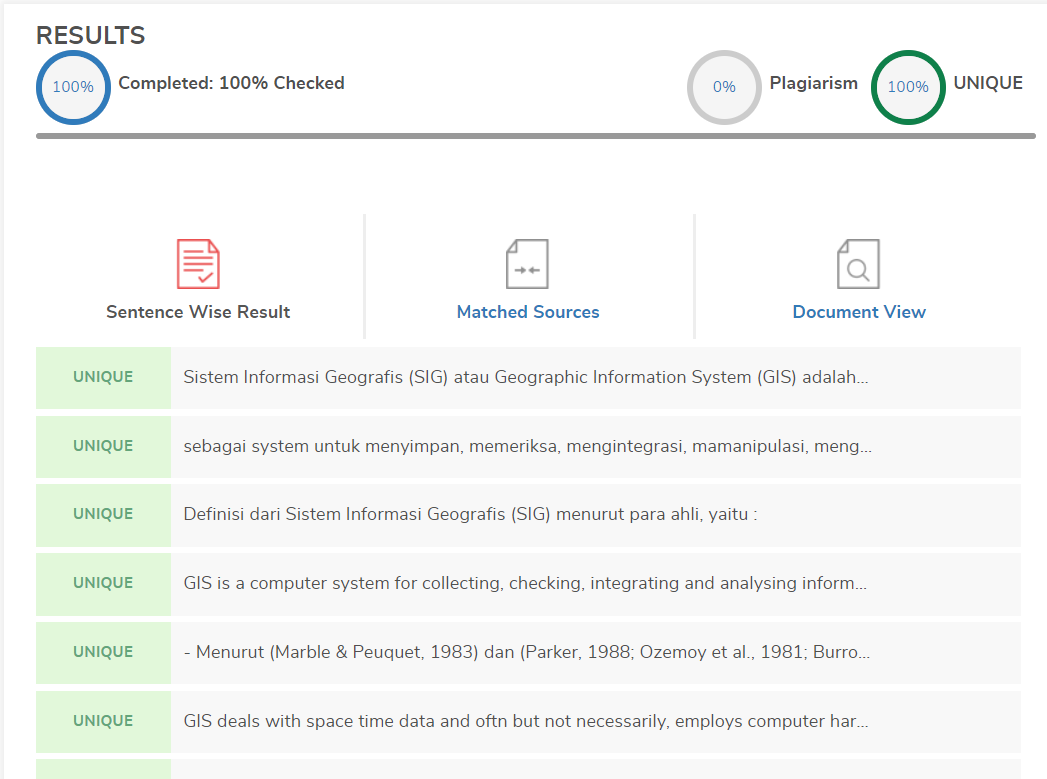
\includegraphics[width=4cm]{figures/Tugas1/1174084/plagiarism.png}
	\centering
	\caption{Plagiarism}
    \end{figure}
 